\documentclass{beamer}
\usepackage[utf8]{inputenc}
\usepackage[T2A]{fontenc}
\usepackage[english,russian]{babel}
\usepackage{graphicx} % Пакет для работы с изображениями
\usepackage{adjustbox} % Hyperlinks
\usepackage{blindtext} % Hyperlinks

\usetheme{default}
% \definecolor{myblue}{RGB}{0,0,0} % Define black color (RGB values)
% \setbeamercolor{frametitle}{fg=myblue} % Set frame title color to black
% \setbeamerfont{frametitle}{series=\bfseries}
\setbeamertemplate{footline}[frame number]

\begin{document}

\begingroup
\setbeamertemplate{footline}{}
\begin{frame}
\begin{center}
    % \hfill
    \begin{minipage}{0.1\textwidth}
        
\includegraphics[width=1.7cm]{img/bmstu_logo.jpg}
    \end{minipage}
    % \hspace{1cm}
    \hfill
    \begin{minipage}{0.80\textwidth}
        {
            Die Moskauer Staatliche

            Technische Bauman-Universit\"at
        }
    \end{minipage}
    % \hfill
\end{center}
\rule[3ex]{\linewidth}{1pt}

\begin{center}
    \huge Softwaretechnik
\end{center}

\vfill

\begin{flushright}
    \begin{minipage}{0.4\textwidth}
        \makebox[1.5cm]{Student: \hfill} Runov K.A.

        \makebox[1.5cm]{Gruppe: \hfill} IU7-64B

        \makebox[1.5cm]{Lehrerin: \hfill} Valitskaya I.L.
    \end{minipage}
\end{flushright}

\vfill

\begin{center}
    26. Februar 2024
\end{center}

\end{frame}
\endgroup

\begin{frame}
\frametitle{Inhalt}
    \begin{enumerate}
            \item<1-> Softwaretechnik
                \begin{itemize}
                    \item<1-> Definition
                    \item<1-> Etappen
                    % \item<1-> Softwarebeispiele
                \end{itemize}
            \item<1-> Disziplinen an der Fakultät für Softwaretechnik
                \begin{itemize}
                    \item<1-> Technishe disziplinen
                    \item<1-> Geisteswissenschaftliche disziplinen
                    % \item<1-> Aufgabenbeispiele
                \end{itemize}
            \item<1-> Vielen Dank
    \end{enumerate}
\end{frame}

\begin{frame}
    \frametitle{Definition von Softwaretechnik}
    \centering
    \vfill
Es gibt keine strikte Definition
    \vfill
\end{frame}

\begin{frame}
    \frametitle{1. Planung und Analyse von Anforderungen}
    % \centering
    \begin{minipage}{0.45\textwidth}
        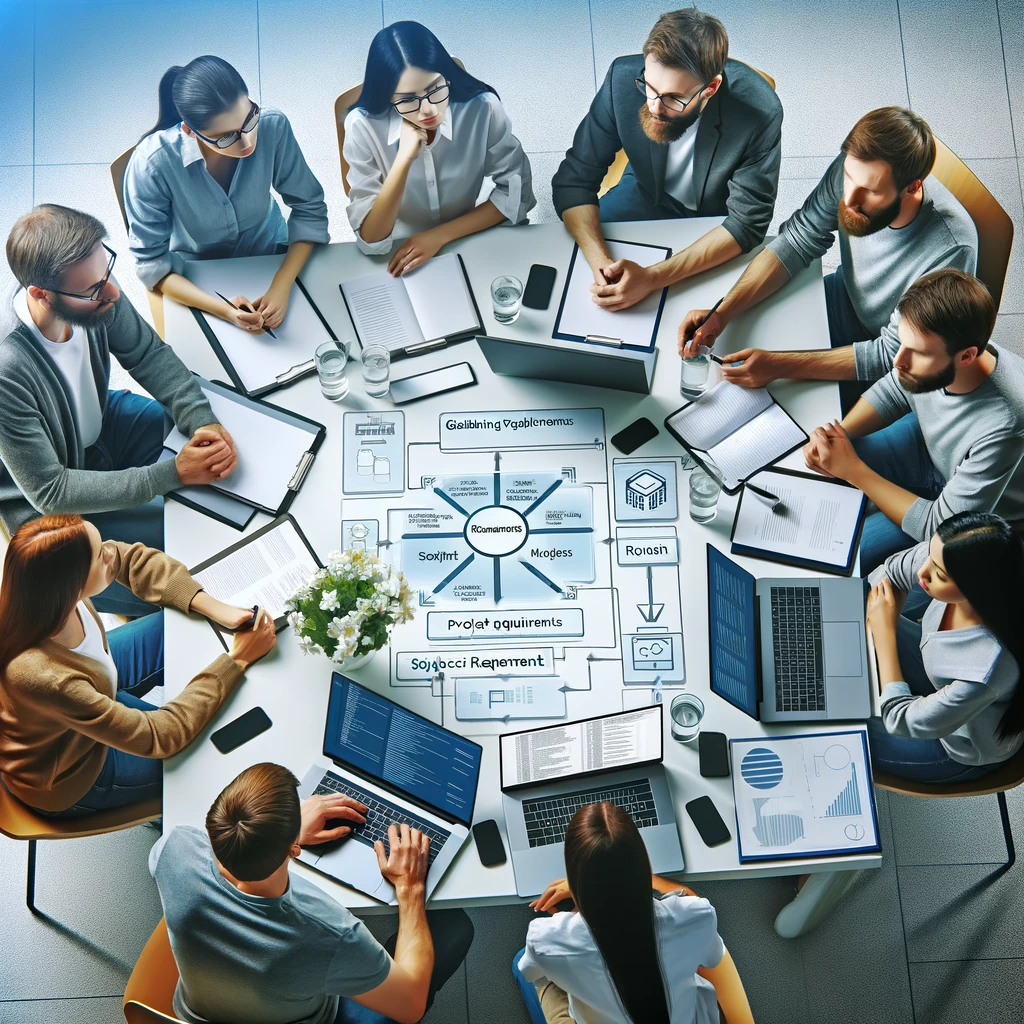
\includegraphics[width=\textwidth]{img/1.png}
    \end{minipage}
    \hfill
    \begin{minipage}{0.45\textwidth}
        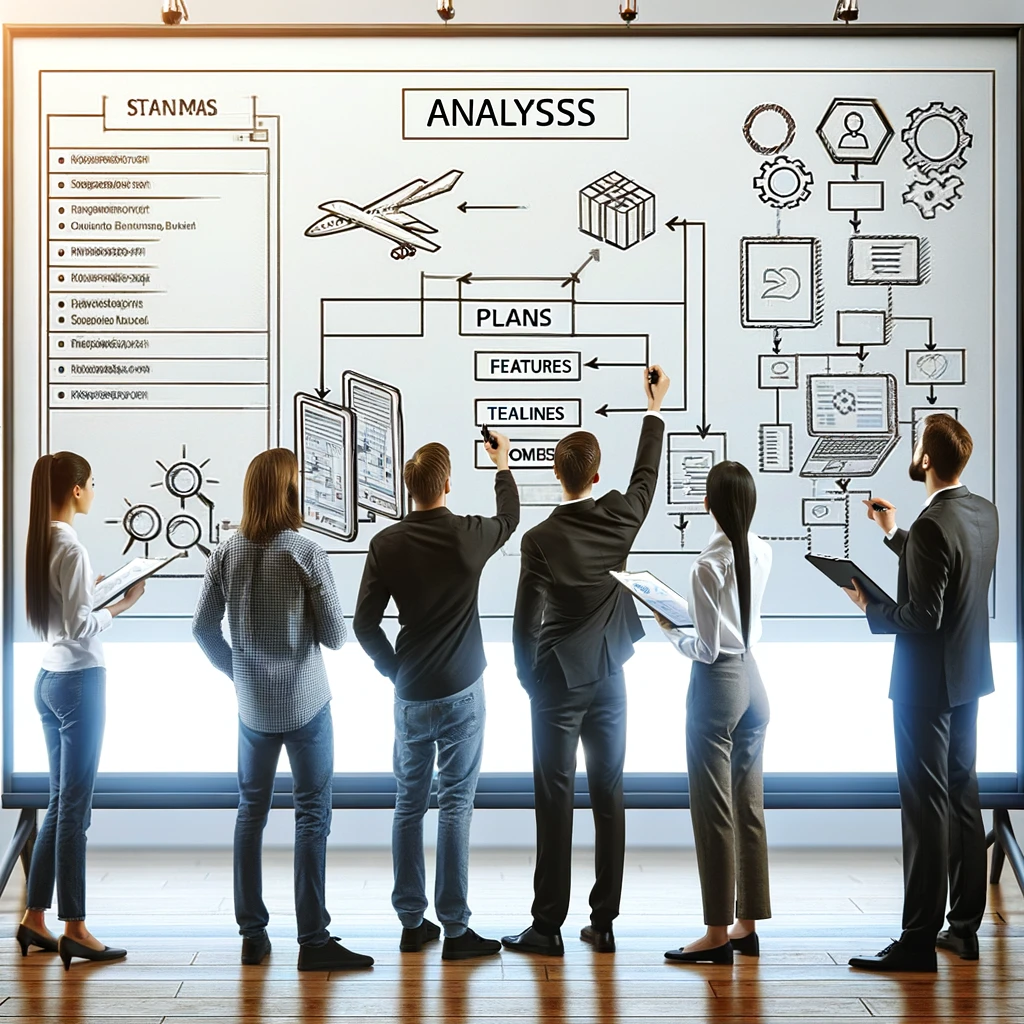
\includegraphics[width=\textwidth]{img/2.png}
    \end{minipage}
\end{frame}

\begin{frame}
    \frametitle{2. Design}
    \centering
    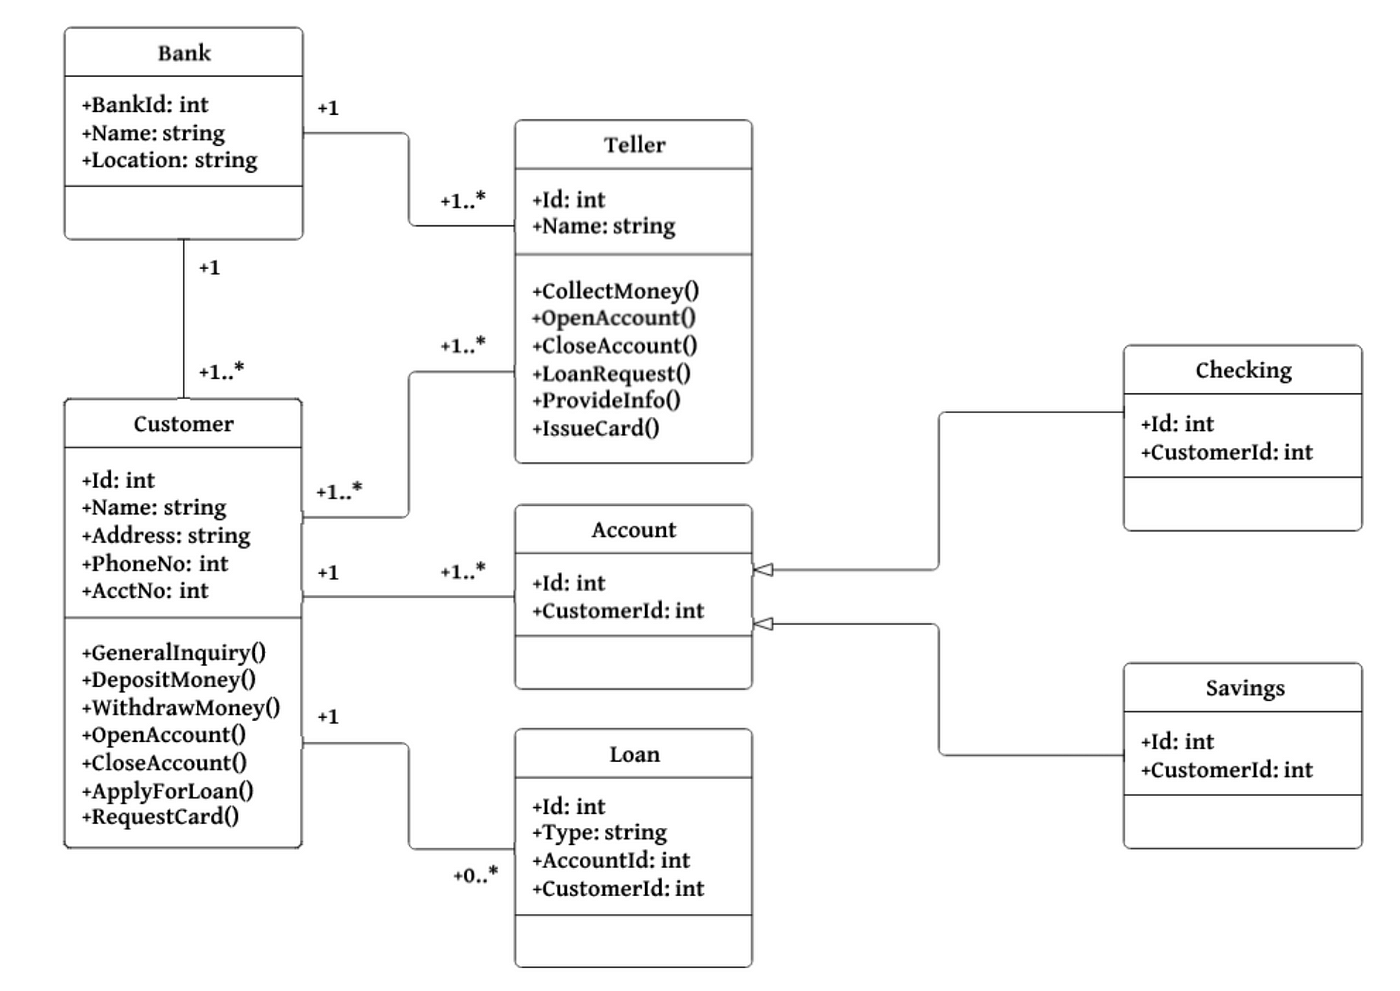
\includegraphics[width=\textwidth]{img/uml.png}
\end{frame}

\begin{frame}
    \frametitle{3. Codeschreiben}
    \centering
    
\includegraphics[width=\textwidth]{img/coding.jpg}
\end{frame}

\begin{frame}
    \frametitle{4. Prüfung und Unterstützung}
    \centering
    
\includegraphics[height=0.9\textheight]{img/debugging.png}
\end{frame}

\begin{frame}
    \frametitle{Fakultät für Softwaretechnik}
    \centering
    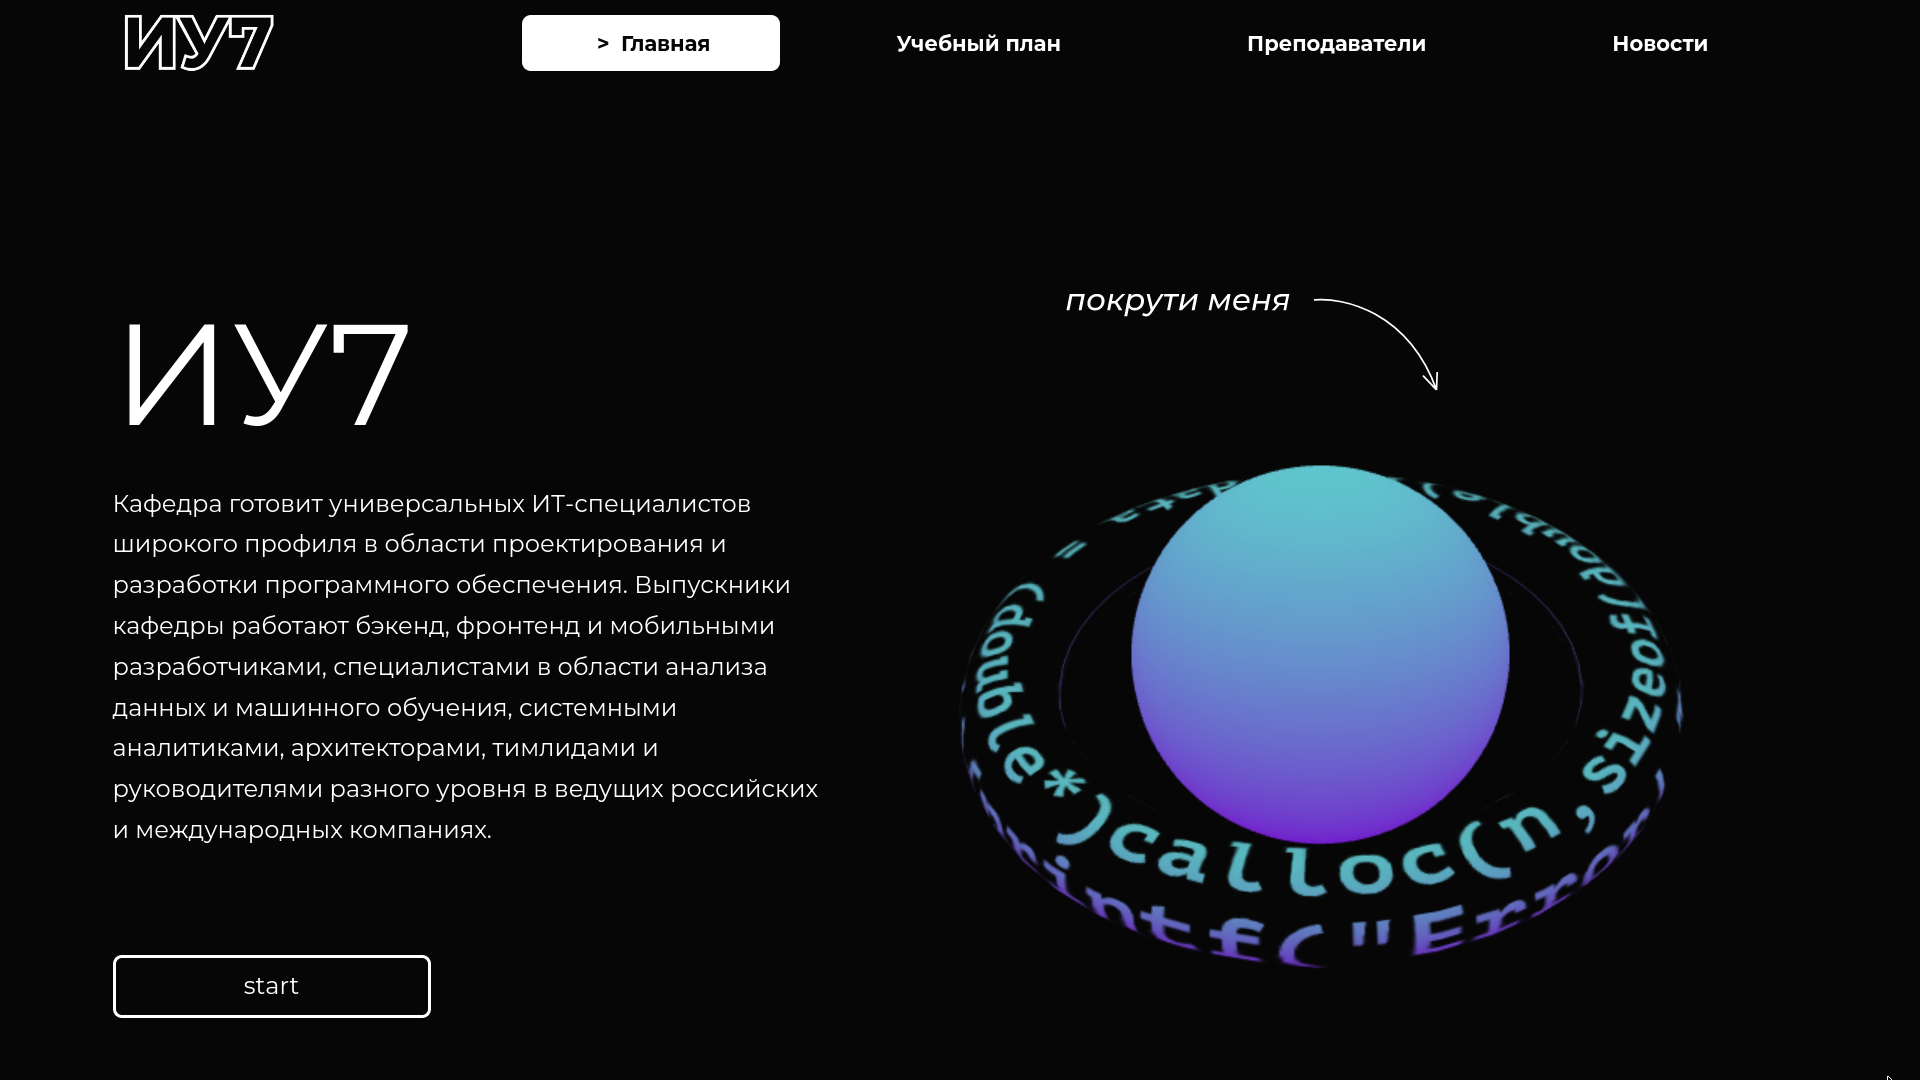
\includegraphics[width=\textwidth]{img/iu7.png}
\end{frame}

\begin{frame}
\frametitle{Technishe disziplinen an der Fakultät für Softwaretechnik}
\begin{minipage}{0.5\textwidth}

\includegraphics[width=\textwidth]{img/good.png}
\end{minipage}
\begin{minipage}{0.45\textwidth}
    \begin{itemize}
        % \item<1-> Матан % (матан, линал, дискра, логика, тервер, матстат)
        % \item<1-> Программирование % (си, ооп, асм, функ, лог)
        % \item<1-> Компьютерная графика
        % \item<1-> Базы данных
        % \item<1-> Типы и структуры данных
        % \item<1-> Анализ алгоритмов
        % \item<1-> Операционные системы
        % \item<1-> Проектирование ПО
        % \item<1-> Моделирование
        % \item<1-> Защита информации
        % \item<1-> Компьютерные сети
        \item<1-> Mathematik
        \item<2-> Programmierung
        \item<3-> Computergrafik
        \item<4-> Datenbanken
        \item<5-> Algorithmusanalyse
        \item<6-> Betriebssystem (OS)
        \item<7-> Software-Design
        \item<8-> Modellierung
        \item<9-> Datenschutz
        \item<10-> Computernetzwerke
        % \item<1-> Datentypen und -strukturen
    \end{itemize}
\end{minipage}
\end{frame}

\begin{frame}
\frametitle{Geisteswissenschaftliche disziplinen an der Fakultät für Softwaretechnik}
\begin{minipage}{0.5\textwidth}
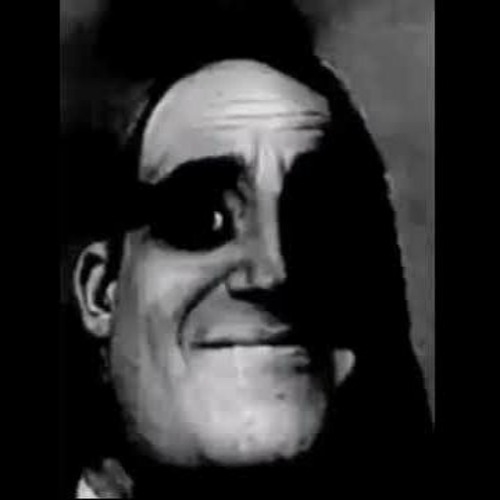
\includegraphics[width=\textwidth]{img/bad.jpg}
\end{minipage}
\begin{minipage}{0.45\textwidth}
    \begin{itemize}
        % \item<1-> Инжграф
        % \item<1-> Физика
        % \item<1-> История
        % \item<1-> Правоведение
        % \item<1-> Политология
        % \item<1-> Социология
        % \item<1-> Экология
        % \item<1-> ОМО
        % \item<1-> Безопасность жизнедеятельности
        % \item<1-> Философия
        \item<1-> Ingenieurgrafiken
        \item<2-> Physik
        \item<3-> Geschichte
        \item<4-> Rechtswissenschaft
        \item<5-> Politologie
        \item<6-> Soziologie
        \item<7-> \"Okologie
        \item<8-> Lebenssicherheit
        \item<9-> Philosophie
        \item<10-> Deutsche
    \end{itemize}
\end{minipage}
\end{frame}

\begingroup
\begin{frame}
    \vfill
\begin{center}
    \huge Vielen Dank f\"ur Ihre Aufmerksamkeit!
\end{center}
    \vfill
\end{frame}
\endgroup

\end{document}
